\section{Topologies for real-time multimedia communication}
\label{sec:topologies}


%% 
%% Leave first page empty
\thispagestyle{empty}

In this chapter we discuss different possible topologies that can be used along in real time media communication.

A topology can be defined as the arrangement of the various nodes of a network together, those nodes can be connected through different links and configurations. Topologies enable different RTC architectures with optimal performance for each specific scenario. 

%In WebRTC, we want to study how they perform in the most common use cases for real time multimedia communication.

Some challenges are common in all the topologies described in this chapter. For example, NAT traversal problems decide either if the call is established or not, this problem can be solved in WebRTC with the usage of TURN and STUN, but in some restrictive environments it might be impossible to succeed with the call establishment. 

The usage of NAT traversal mechanisms in WebRTC is crucial and at the same time it increases the complexity of the browser internals. STUN and TURN servers must be reachable from the browser perspective in order to provide the ports and IP alternatives to connect, those are gathered into {\it candidates} that are evaluated by the ICE on the browser. ICE proceeds with the best option to perform the connection. 

All the previous mechanisms are supposed to provide high level of success probability but might fail in very restrictive environments. To solve some of the issues, WebRTC allows UDP and TCP (using TURN) packet transport, this is done to enable connectivity even in very restrictive environments that could have UDP packet drop mechanisms. 

For some topologies that include the establishment of multiple {\it PeerConnections} resource usage can be a big problem (e.g. mesh, one-to-many or tree). Considering that system capacity relies in how the OS architecture handles processes, CPU and memory usage of WebRTC might be seen as a constraint for those topologies. For example, in Unix based systems every tab of a browser is treated as a separate process meanwhile in other architectures this might be handled different. Media encoding usually consume most of those resources becoming a bottleneck for some scenarios.

\subsection{Point-to-Point}

The simplest topology is a permanent session between two peers, this model is widely used in telephony and provides reliable real time communication between users. In WebRTC, point-to-point topologies work only within people in the same domain opposite to many cross-domain communication alternatives such as SIP. Scenarios such as Figure~\ref{fig:SIParchitecture} are difficult to design in a WebRTC application, on the other side, Figure~\ref{fig:webrtcExample} represents the most common WebRTC point-to-point scenario.

With point-to-point topology we can have traditional dedicated paths where the resources are reserved for each call. In small Local Area Networks (LAN) \nomenclature{LAN}{Local Area Networks} we use dedicated paths between two WebRTC users, this path can go through the switch or relay but it is unlikely that is going to change the routing. For WebRTC calls over the public internet, the route can change at any time trying to use the optimal path, this is done in packet-switching technologies where the route is set up dynamically. However, the user perception is that the communication is done end-to-end without noticing any change on the network nodes. 

From usability perspective, different environments might require point-to-point topologies, direct calls between two users or real time communication for IM can be possible scenarios. 

%Use cases examples for point-to-point topologies allow communication between doctor and patient in a medical web application that is cross-platform compatible and uses an WebRTC. Communication in other cases such as citizens and authorities could also succeed in a WebRTC application.
 
\subsection{One-to-Many}

One-to-many or star topologies are one of the most common network topologies for media streaming (e.g Windows Media Server or RTMFP), this kind of topology consist on a central node that transmits streams to the rest of nodes connected to it. In the WebRTC example of Figure~\ref{fig:starExample}, the central node might be also receiving real time data in difference of the traditional streaming scenarios providing P2P communication between the peers and the central node.

 \begin{figure}[h]
  \centering
    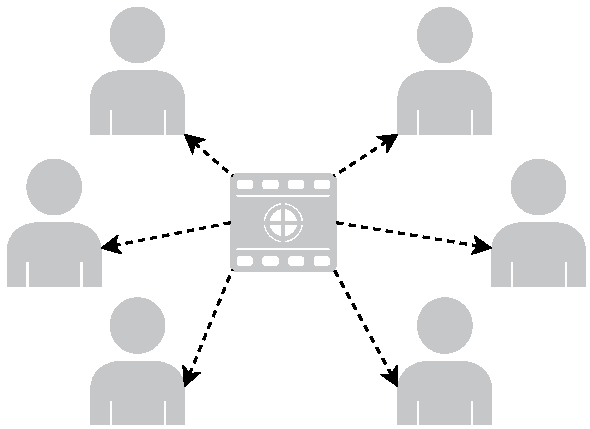
\includegraphics[width=0.5\textwidth]{./figures/star.pdf}
      \caption[One-to-many topology for real time media]{One-to-many topology for real time media.}
	\label{fig:starExample}
\end{figure}

Star scenarios are known as a type of multicast, one source sends the media to the different clients that connect to the origin. When using this topology, the common uses are related with video and audio streaming to multiple peers, TV media and streaming conferences are popular use cases.

Live streaming is a common in-demand scenario for internet TV channels, this topology adapts to the requirements of the providers as subscribers can join the suggested channel when desired. 

Some of the problems are: high dependency of the central node and, in case of failure, the central node streaming could stop loosing all connectivity with the peers. On the other side, this topology is also good as it provides reliability in case of failure of one of the connected nodes because the rest of the network won't notice any difference on the response. 

For example, we could have a major sport even being retransmitted to the viewers by using one-to-many. Other solutions could cover the use of WebRTC to have a CEO talking to the employees with an HMTL5 web application. Music bands also could take advantage of this scenario by being able to transmit his show to the audience with feedback in real time or having the members playing from different geographic areas. All the previous examples take advantage of WebRTC by having direct feedback from the connected nodes, actual media streaming technologies do not provide this kind of communication between the viewer and the origin.

%\subsubsection{Challenges}
In star topology we have a video, audio and data streaming connection from one source to multiple devices. This might cause a huge load on the source when having multiple {\it PeerConnection} running, central node performance can be a big constraint in this scenario. Observing other topologies, in most cases, media delay on the network is not as important as other options due to the one-way communication only. In most scenarios, video and audio is not required to be received on the source, so having the media delayed a couple of seconds is not going to affect the user experience in the call. Those scenarios are one-way only use cases.

From the client perspective, the {\it PeerConnection} stablished is easy to handle as  in most cases no data is going to be sent back to the source, except the RTCP control messages.

\subsection{Many-to-Many}

Many-to-many topologies are also known as mesh, this style of topology is used in multiple VoIP systems for conferencing purposes. Conferencing systems are widely extended in enterprises for long-distance communication between employees and working groups, by this, the need of having those calls working with good response for all participants is very important.

In a full mesh topology all peers connect between them increasing the number of connections and used resources. The value of fully meshed networks rely on the number of subscribers, the amount of {\it PeerConnections} stablished in a mesh network shall be dependent on the amount of people in the conference. The number of {\it PeerConnections} can grow rapidly based on Equation~\ref{eq:meshformula}.

\begin{equation}
	\label{eq:meshformula}
	c = \frac{n(n-1)}{2}\\
	
	c \text{: Number of {\it PeerConnections}}\
		
	n \text{: Nodes in the mesh}
\end{equation}

Equation~\ref{eq:meshformula} calculates the amount of WebRTC connections required for a {\it full mesh} topology. 

\subsection{Multipoint Control Unit (MCU)}

MCU \nomenclature{MCU}{Multipoint Control Unit} is a device used to bridge streams in conferences, it multiplexes, mixes and encodes media of different sources to be sent over one gateway. MCU usage could be a good alternative when designing WebRTC infrastructures such as video conferencing, the ability to multiplex different streams into the same channel is going to directly affect on how the client performs when reproducing the video.

In real time media topologies, MCU is a common component, used as relay it helps end devices to handle less load for the sources by multiplexing all the streams of the call into the same channel, we can have multiple peers connected to the same MCU that can multiplex the media sent by all of them into one unique stream forwarded to all the participants of the call.

MCUs receive the streams from the clients and multiplex them over one unique channel, this provides good scalability from the client perspective because it is only building one connection even there are multiple peers on the conference.

Some MCUs may have to encode and decode media on the fly, this is can be difficult in real time applications but can provide different encoding options to adapt the stream output to the link conditions. Usually transcoding is not suitable for real time environments.

Drawbacks on the MCU model affect the dependency of the end nodes from the MCU, if the MCU fails to give good latency and performance, the call quality is affected and receivers do not get the expected response. Load in the MCU can be very high when multiple conferences are being stablished, this requires abundant resources and good throughput.

Point-to-point topologies do not require much resources from the service provider, but for the MCU scenario the service provider has to be able to scale properly.

\subsection{Overlay}

Overlaying media streams is the ability of a peer to forward media to a third party. Topologies that use overlay are those that require the media to be forwarded from one peer to the other, this kind of behavior is given in multiple peer topologies such as {\it hub-spoke} or {\it tree}, seen in Figure~\ref{fig:overlaytopologies}.

Generally, in multiple peer scenarios, we can combine all of the following structures to build a topology that fit our requirements.

WebRTC does not provide native support for media overlay yet, but it is planned to implement those features in future versions of the API. Traditionally overlay has also been used for media streaming over the internet.

\begin{figure}[h]
        \centering
        \begin{subfigure}[b]{0.5\textwidth}
                \centering
                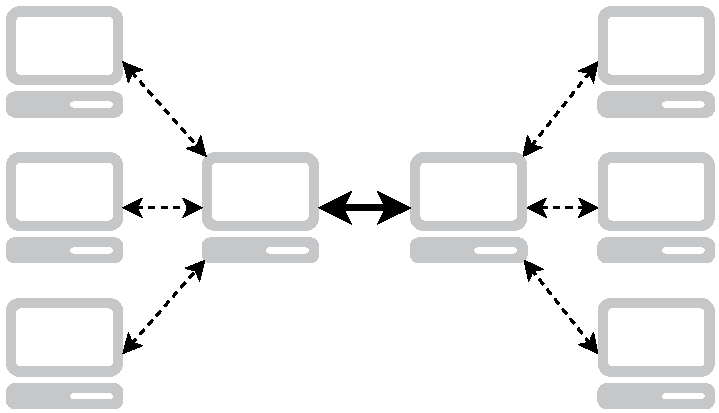
\includegraphics[width=\textwidth]{./figures/hubandspoke.pdf}
                \caption{Hub-spoke topology}
                \label{fig:hubandspoke}
        \end{subfigure}%
        ~ %add desired spacing between images, e. g. ~, \quad, \qquad etc.
          %(or a blank line to force the subfigure onto a new line)
        \begin{subfigure}[b]{0.5\textwidth}
                \centering
                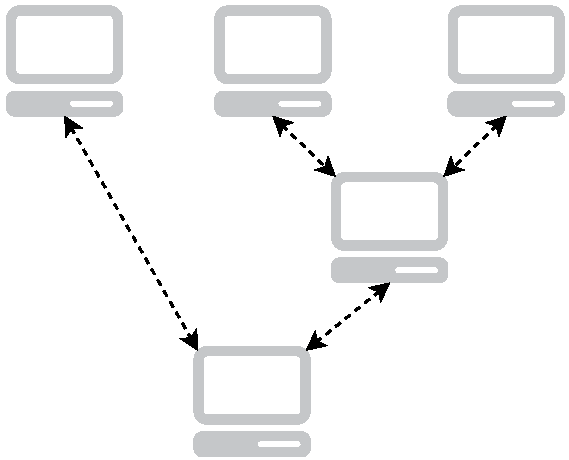
\includegraphics[width=\textwidth]{./figures/three.pdf}
                \caption{Tree topology}
                \label{fig:three}
        \end{subfigure}
        \caption[Overlay topologies]{Overlay topologies.}
        \label{fig:overlaytopologies}
\end{figure}

\subsubsection{Hub-spoke}

Hub-spoke distribution is a topology composed by nodes and arranged like a chariot wheel. Traffic moves along spokes that are connected to the hub at the center. This type of topology, represented in Figure~\ref{fig:hubandspoke}, is good for some scenarios as it requires less connections to perform a full mesh communication in the network. 

This is a centralized model, we might have problems if the key nodes of the topology fail. It also relies in one or multiple trunk paths that can be crucial for the success of the streaming, those paths should provide good throughput and low delay.

In some technologies that rely in hub and spoke, the central nodes are usually picked from the end users, calculating the best response from the users the system is able to select the best candidate where the rest of nodes connect to. When this happens that node is handling and forwarding more data that in a standalone call, sometimes without knowledge.

This topology uses the concept of overlay previously described. Hub-spoke environments are also used for logistics in the world, for delivering products and goods around the globe, focusing in bridges over the continents, goods in Europe are distributed within an internal network and shipped to other continents from a centralized node.  

\subsubsection{Tree}
 
Tree topology is based on a node hierarchy, the highest level of the tree consist of a single node that is connected to one or more nodes that forward the traffic to the other layers of the topology. Tree topologies are not constrained by the number of levels and can adapt to the required amount of end users as seen in Figure~\ref{fig:three}.  

This type of topologies are scalable and manageable. In case of failure it is relatively easy to identify the broken branch of the tree and repair that node.

On the other side, we can have connectivity problems if a node fails to keep the link up, all the layers under that node are going to be affected and the media forwarding will stop. Overlay is crucial for this topology that is widely used in media streaming, for real time communications, large tree topologies won't be the best candidates given the delay produced when forwarding the packets.

Topologies such as tree are not only used for media streaming but they can also be used to provide wireless coverage in difficult areas, acting as hotspots, each hop can extend the coverage of the wireless in remote areas.

